\documentclass{article}
\usepackage{tikz}  % Biblioteca TikZ para gráficos
\usepackage{todonotes}

%www.tikzmaker.com




\begin{document}

% Ejemplo 1: Línea Recta
\section*{Ejemplo 1: Línea Recta}
\begin{figure}[h!]
    \centering
    \begin{tikzpicture}
        % Dibuja una línea desde el punto (0,0) hasta el punto (4,2)
        \draw[thick] (0,0) -- (4,2);
    \end{tikzpicture}
    \caption{Línea recta desde (0,0) a (4,2).}
\end{figure}

\todo[caption={Importante}]{Asegúrate de que los resultados sean coherentes.} % Nota con un título

% Ejemplo 2: Cuadrícula
\section*{Ejemplo 2: Cuadrícula}
\begin{figure}[h!]
    \centering
    
\begin{tikzpicture}
        % Dibuja una cuadrícula de 5x5 con líneas de separación cada 1 unidad
        \draw[step=1cm, gray, very thin] (0,0) grid (5,5);
    \end{tikzpicture}
    \caption{Cuadrícula de 5x5 con líneas cada 1 cm.}
\end{figure}

% Ejemplo 3: Círculo y Punto
\section*{Ejemplo 3: Círculo y Punto}
\begin{figure}[h!]
    \centering
    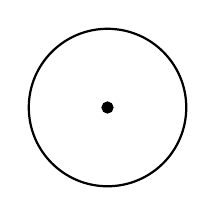
\begin{tikzpicture}
        % Dibuja un círculo con radio 1 y un punto en el centro
        \draw[thick] (0,0) circle (1cm);      % Círculo de radio 1 cm
        \filldraw (0,0) circle (2pt);         % Punto en el centro
    \end{tikzpicture}
    \caption{Círculo con un punto en el centro.}
\end{figure}
\todo[inline, color=blue!30]{holaaaaaaaaaaaaaaaaaa}

\begin{figure}[h!]
    \centering
    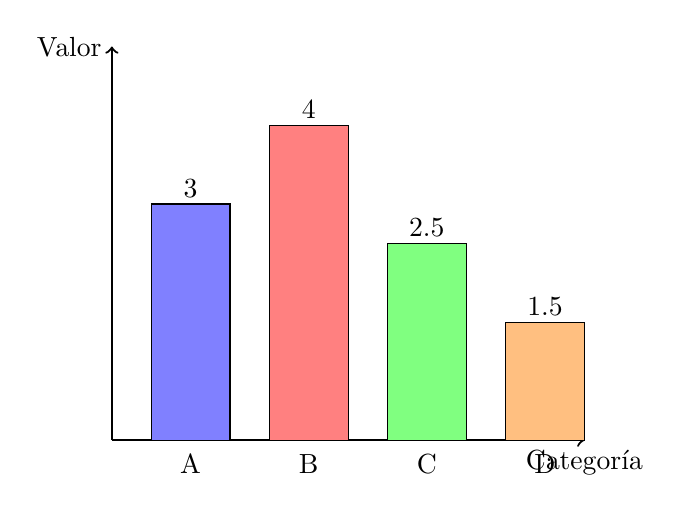
\begin{tikzpicture}
        % Ejes
        \draw[thick, ->] (0,0) -- (6,0) node[anchor=north] {Categoría};
        \draw[thick, ->] (0,0) -- (0,5) node[anchor=east] {Valor};

        % Barras
        \draw[fill=blue!50] (0.5,0) rectangle (1.5,3);
        \draw[fill=red!50] (2,0) rectangle (3,4);
        \draw[fill=green!50] (3.5,0) rectangle (4.5,2.5);
        \draw[fill=orange!50] (5,0) rectangle (6,1.5);

        % Etiquetas de las barras
        \node at (1,3.2) {3};
        \node at (2.5,4.2) {4};
        \node at (4,2.7) {2.5};
        \node at (5.5,1.7) {1.5};

        % Nombres de las categorías
        \node at (1, -0.3) {A};
        \node at (2.5, -0.3) {B};
        \node at (4, -0.3) {C};
        \node at (5.5, -0.3) {D};
    \end{tikzpicture}
    \caption{Gráfico de barras con cuatro categorías.}
\end{figure}
\newpage


\section*{Gráfico de Función}

\begin{figure}[h!]
    \centering
    \begin{tikzpicture}
        % Ejes
        \draw[->] (-3.5,0) -- (3.5,0) node[anchor=north] {x};
        \draw[->] (0,-2) -- (0,5) node[anchor=east] {y};

        % Gráfico de la función
        \draw[domain=-3:3, smooth, variable=\x, blue, thick] 
            plot ({\x}, {\x*\x}) node[anchor=south] {$y = x^2$};

        % Puntos en la función
        \filldraw[red] (1,1) circle (2pt) node[anchor=south west] {$(1,1)$};
        \filldraw[red] (2,4) circle (2pt) node[anchor=south west] {$(2,4)$};
    \end{tikzpicture}
    \caption{Gráfico de la función \( y = x^2 \).}
\end{figure}



\end{document}

